% =============================================================================
%  Séance 4 — Pré-traitement et géodatabase PostGIS
%  Projet « Accès aux soins — région Casablanca-Settat » (Géodata appliquée)
%
%  Mise en page identique à la présentation de la séance 3 (XeLaTeX / pdfLaTeX).
% =============================================================================
\documentclass[aspectratio=169,10pt]{beamer}

\usepackage{iftex}
\ifPDFTeX
  \usepackage[T1]{fontenc}
  \usepackage[utf8]{inputenc}
\fi
\usepackage[french]{babel}
\frenchsetup{AutoSpacePunctuation=false}
\usepackage[sfdefault]{FiraSans}
\usepackage[scaled=0.86]{FiraMono}
\usepackage{booktabs}
\usepackage{tabularx}
\usepackage{array}
\usepackage{graphicx}
\usepackage{xcolor}
\usepackage{tikz}
\usetikzlibrary{arrows.meta,positioning,calc,fit}

\graphicspath{{../preuves/}{../docs/uml/}{preuves/}{uml/}}
\AtBeginDocument{\hyphenpenalty=10000 \exhyphenpenalty=10000}

% --- Palette -----------------------------------------------------------------
\definecolor{encre}{HTML}{14232E}
\definecolor{bleu}{HTML}{2B7BB9}
\definecolor{sarcelle}{HTML}{1E8A80}
\definecolor{ambre}{HTML}{C8742A}
\definecolor{rouge}{HTML}{C0392B}
\definecolor{gris}{HTML}{6B7280}
\definecolor{fond}{HTML}{F1F4F7}
\definecolor{ligne}{HTML}{D9DEE3}

% --- Mise en page ------------------------------------------------------------
\setbeamersize{text margin left=13mm, text margin right=13mm}
\setbeamertemplate{navigation symbols}{}
\setbeamercolor{normal text}{fg=encre, bg=white}
\setbeamercolor{structure}{fg=bleu}
\setbeamercolor{alerted text}{fg=ambre}
\setbeamertemplate{itemize item}{\textcolor{sarcelle}{\rule[0.35ex]{0.75ex}{0.75ex}}}
\setbeamertemplate{itemize subitem}{\textcolor{gris}{--}}
\setbeamertemplate{enumerate item}{\textcolor{sarcelle}{\bfseries\insertenumlabel.}}

\setbeamertemplate{background}{%
  \begin{tikzpicture}
    \useasboundingbox (0,0) rectangle (\paperwidth,\paperheight);
    \fill[sarcelle] (0,0) rectangle (1.6mm,\paperheight);
  \end{tikzpicture}}

\setbeamertemplate{frametitle}{%
  \vskip5mm
  {\color{ambre}\scriptsize\bfseries\MakeUppercase{\insertsectionhead}}\par
  \vskip0.8mm
  {\color{encre}\Large\bfseries\insertframetitle}\par
  \vskip1.6mm
  {\color{ligne}\rule{\linewidth}{0.6pt}}}

\setbeamertemplate{footline}{%
  \hspace*{13mm}{\color{gris}\tiny Accès aux soins — Casablanca-Settat \enskip·\enskip
  Séance 4 — Pré-traitement et géodatabase PostGIS}\hfill
  {\color{gris}\tiny\bfseries\insertframenumber\,/\,\inserttotalframenumber}\hspace*{13mm}
  \vskip4mm}

\newcommand{\ok}{\textcolor{sarcelle}{\bfseries\checkmark}}
\newcommand{\code}[1]{{\ttfamily\small #1}}
\newcommand{\petit}[1]{{\footnotesize\color{gris}#1}}

\newcommand{\kpi}[4]{%
  \begin{tikzpicture}[baseline=(k.north)]
    \node[fill=fond, rounded corners=3pt, text width=1.95cm, minimum height=2.45cm,
          align=left, inner sep=2.3mm, anchor=north west] (k) at (0,0)
      {\raggedright\spaceskip=0.25em plus 0.05em {\color{#1}\fontsize{15}{17}\selectfont\bfseries #2}\\[1.2mm]
       {\footnotesize\bfseries #3}\\[0.3mm]{\scriptsize\color{gris} #4}};
    \fill[#1] (k.north west) rectangle ($(k.south west)+(0.9mm,0)$);
  \end{tikzpicture}}

\newcommand{\commande}[1]{%
  \begin{tikzpicture}
    \node[fill=encre, rounded corners=3pt, text width=\linewidth-6mm, inner sep=3mm,
          align=left, text=white] {\ttfamily\small #1};
  \end{tikzpicture}}

\newcommand{\partie}[3]{%
  \section{#2}
  {\setbeamertemplate{background}{%
     \begin{tikzpicture}
       \useasboundingbox (0,0) rectangle (\paperwidth,\paperheight);
       \fill[encre] (0,0) rectangle (\paperwidth,\paperheight);
       \fill[sarcelle] (0,0) rectangle (1.6mm,\paperheight);
     \end{tikzpicture}}
   \begin{frame}[plain]
     \vspace*{12mm}
     {\color{ambre}\fontsize{60}{60}\selectfont\bfseries #1}\par\vskip5mm
     {\color{white}\fontsize{26}{30}\selectfont\bfseries #2}\par\vskip3mm
     {\color{white!65!encre}\large #3}
   \end{frame}}}

\begin{document}

% ---------------------------------------------------------------- Couverture --
{\setbeamertemplate{background}{%
   \begin{tikzpicture}
     \useasboundingbox (0,0) rectangle (\paperwidth,\paperheight);
     \fill[encre] (0,0) rectangle (0.50\paperwidth,\paperheight);
     \fill[sarcelle] (0,0) rectangle (1.6mm,\paperheight);
     \node at (0.75\paperwidth,0.5\paperheight)
       {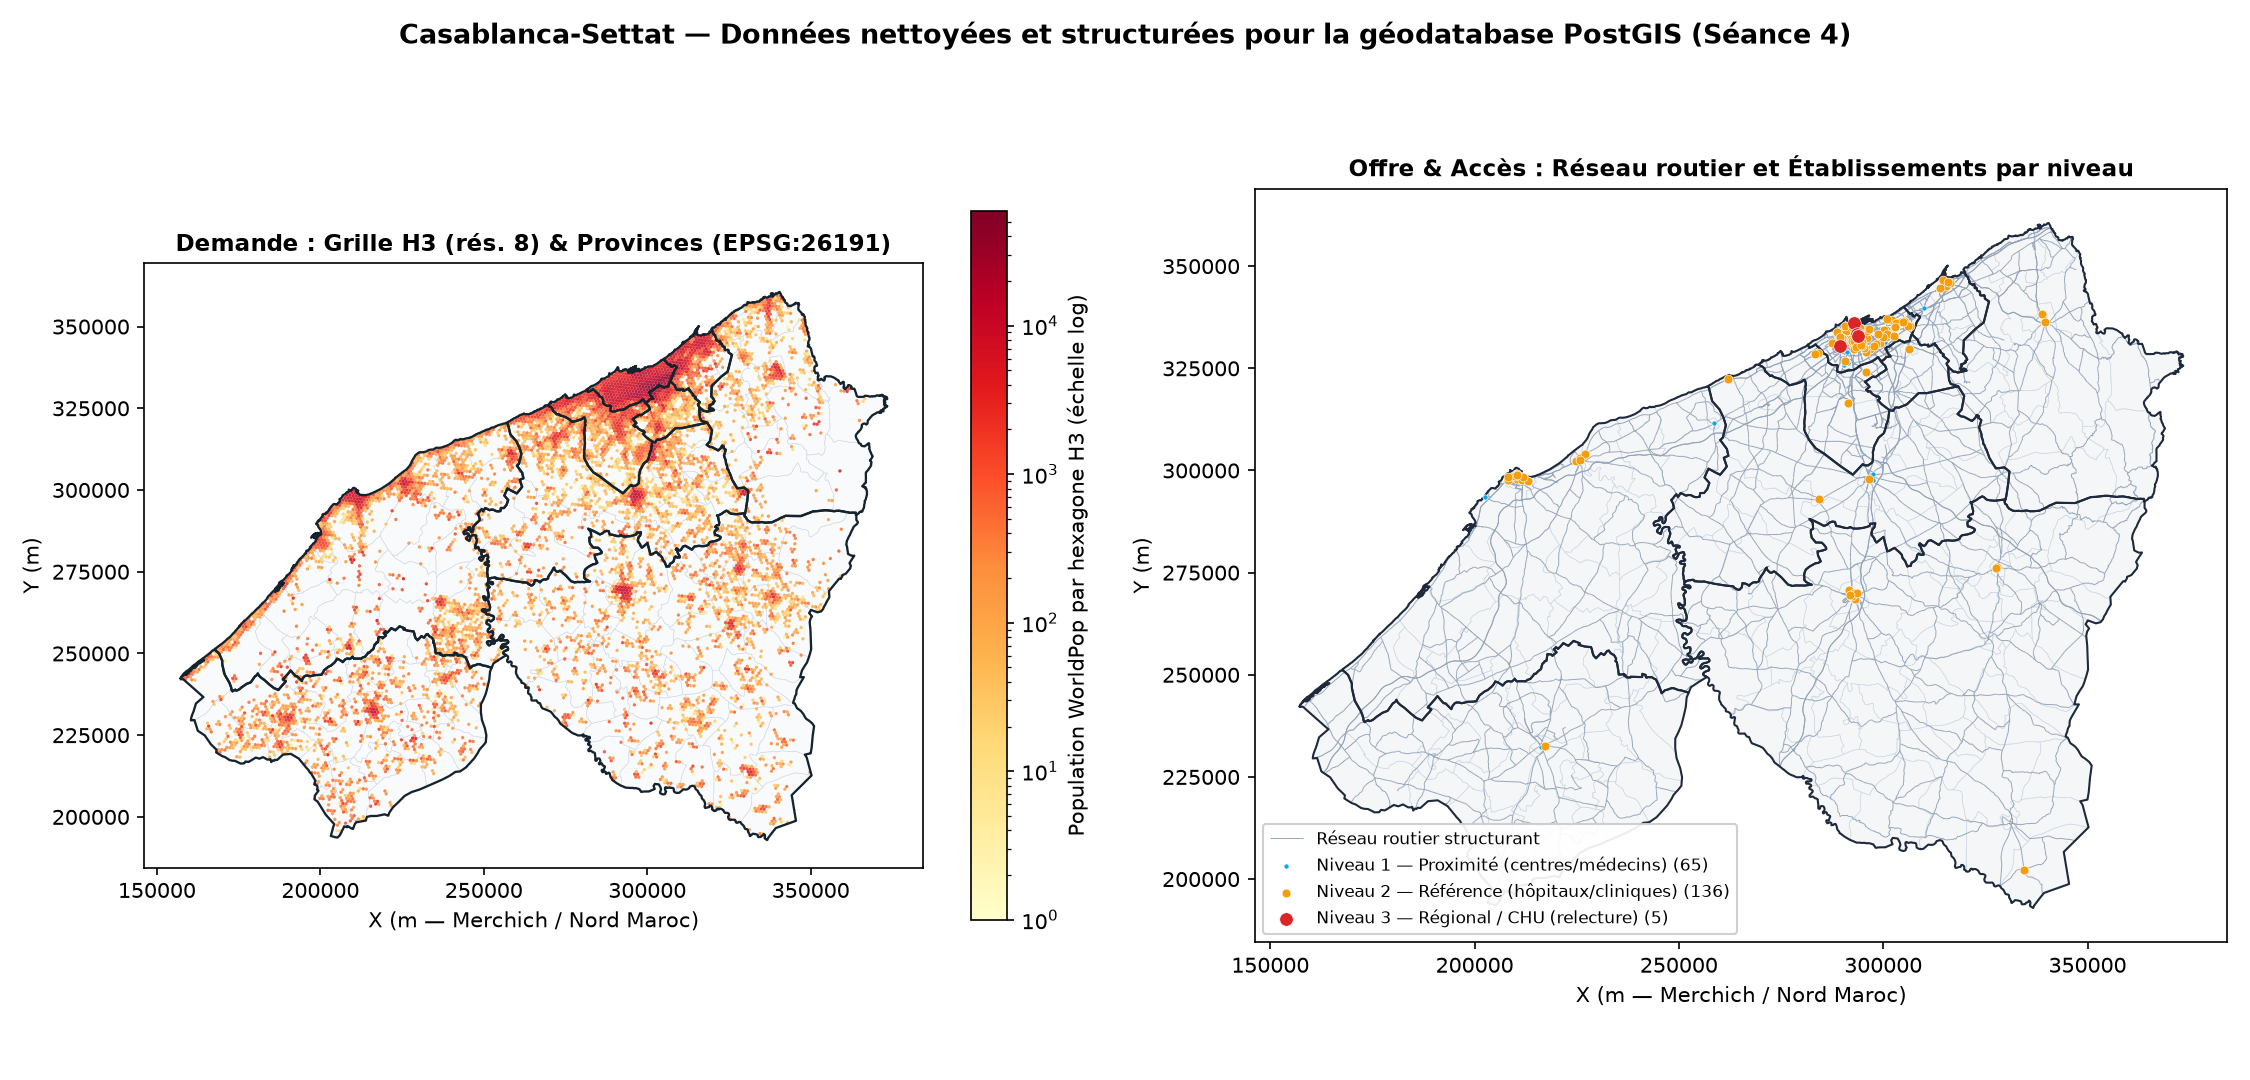
\includegraphics[width=0.46\paperwidth]{carte_nettoyage.png}};
   \end{tikzpicture}}
 \begin{frame}[plain]
   \begin{minipage}[t]{0.38\paperwidth}
     \raggedright
     \vspace*{8mm}
     {\color{ambre}\scriptsize\bfseries GÉODATA APPLIQUÉE · SÉANCE 4}\par\vskip5mm
     {\color{white}\fontsize{20}{24}\selectfont\bfseries Accès aux soins dans la région Casablanca-Settat}\par\vskip4mm
     {\color{white!75!encre}\large Pré-traitement, validation topologique\\ et géodatabase PostGIS}\par\vskip10mm
     {\color{white}\scriptsize
       SOUILAH Meryem · MANYANI Hiba · ZOUHRI Imane\\[0.6mm]
       BELMOKHTARE Fatima Ezzahra · GUEROUANE Imane}\par\vskip2mm
     {\color{white!55!encre}\scriptsize Élèves ingénieurs 3\textsuperscript{e} année}
   \end{minipage}
 \end{frame}}

% ---------------------------------------------------------------------- Plan --
\begin{frame}{Déroulé de la présentation}
  \vskip3mm
  \begin{tikzpicture}[x=1cm,y=1cm]
    \foreach \n/\t/\s [count=\i from 0] in {
        01/{Rappel du défi et cahier des charges}/{question spatiale, attendus de l'intersession 3},
        02/{Nettoyage et désaccords topologiques}/{mode --dry-run, doublons point/polygone, graphe routier, H3},
        03/{Modèle de données (MCD / MLD) et PostGIS}/{8 tables, 10 clés étrangères, contraintes CHECK, index GIST},
        04/{Requêtes spatiales métier et performances}/{3 requêtes pour la séance 5, plans EXPLAIN ANALYZE},
        05/{Démonstration live et sauvegarde}/{rejet FK/SRID en direct, pg\_dump et restauration testée}} {
      \node[anchor=west, text=ambre, font=\Large\bfseries] at (0,-1.05*\i) {\n};
      \node[anchor=west, font=\large\bfseries] at (1.4,-1.05*\i+0.13) {\t};
      \node[anchor=west, font=\footnotesize, text=gris] at (1.4,-1.05*\i-0.3) {\s};
      \draw[ligne] (0,-1.05*\i-0.6) -- (13.4,-1.05*\i-0.6);
    }
  \end{tikzpicture}
\end{frame}

% =============================================================================
\partie{01}{Le défi et la phase}{De la donnée brute à une géodatabase PostGIS intègre et interrogeable}

\begin{frame}{Ce que demandait l'intersession 3 (Séance 4)}
  \small
  \renewcommand{\arraystretch}{1.25}
  \begin{tabularx}{\linewidth}{@{}>{\raggedright\arraybackslash}X>{\raggedright\arraybackslash}p{5.0cm}c@{}}
    \toprule
    \textbf{Consigne} & \textbf{Notre réalisation} & \\
    \midrule
    Détection/correction des géométries invalides, doublons, hors emprise & \code{nettoyage.py} + \code{ST\_MakeValid} (100\,\% valides) & \ok \\
    Mode « rapport seul » (\code{--dry-run}) et rapport avant/après & \code{preuves/rapport\_nettoyage.md} & \ok \\
    Cas réel de désaccord topologique du thème traité & Doublons point/polygone OSM (35 m) + nœuds/boucles routières & \ok \\
    DDL PostGIS normalisé, clés étrangères, import \code{ogr2ogr}, index \code{GIST} & \code{sql/schema.sql} (8 tables, 10 FK, 6 GIST, 10 B-tree) & \ok \\
    3 requêtes spatiales métier utiles pour la séance 5 + \code{EXPLAIN ANALYZE} & \code{sql/requetes.sql} (6,5 ms ; 355 ms ; 1,2 s) & \ok \\
    Base peuplée, dump restaurable et test de restauration & \code{sql/acces\_soins.backup} (42,1 Mo, \code{pg\_restore} validé) & \ok \\
    \bottomrule
  \end{tabularx}
\end{frame}

% =============================================================================
\partie{02}{Nettoyage et topologie}{Un pipeline automatisé avec mode \code{--dry-run} et rapport avant/après}

\begin{frame}{Bilan chiffré avant / après nettoyage (\code{EPSG:26191})}
  \vskip1mm
  \kpi{bleu}{153}{communes}{9 provinces, 153/153 HCP}\hfill
  \kpi{rouge}{1\,583}{établissements}{8 doublons topo fusionnés}\hfill
  \kpi{gris}{318\,229}{arcs routiers}{228\,554 nœuds, 99,8\,\% connexes}\hfill
  \kpi{ambre}{25\,255}{mailles H3}{rés.\ 8, 7\,113 peuplées}\hfill
  \kpi{sarcelle}{100\,\%}{géom.\ valides}{0 invalide, 0 hors région}
  \vskip4mm
  \scriptsize
  \renewcommand{\arraystretch}{1.2}
  \begin{tabularx}{\linewidth}{@{}>{\raggedright\arraybackslash}Xrrrrrc@{}}
    \toprule
    \textbf{Table cible} & \textbf{Avant} & \textbf{Invalides} & \textbf{Doublons} & \textbf{Hors région / boucles} & \textbf{Après} & \textbf{Statut} \\
    \midrule
    \code{province} (dissolution communes) & 153 comm. & $0 \to 0$ & 0 & fermeture $\pm 5\text{ m}$ & \textbf{9} & \ok \\
    \code{commune} + pop.\ RGPH 2024 & 153 & $0 \to 0$ & 0 & 0 & \textbf{153} & \ok \\
    \code{etablissement} (OSM santé) & 1\,737 & $0 \to 0$ & 8 (topo) & 146 hors région & \textbf{1\,583} & \ok \\
    \code{troncon} (graphe routier) & 130\,783 voies & $0 \to 0$ & 0 & 196 boucles & \textbf{318\,229} & \ok \\
    \code{noeud} (intersections) & non topol. & $0 \to 0$ & — & 532 en îlots isolés & \textbf{228\,554} & \ok \\
    \code{maille\_h3} (demande rés.\ 8) & 26\,789 & $0 \to 0$ & 0 & 1\,534 hors région & \textbf{25\,255} & \ok \\
    \bottomrule
  \end{tabularx}
\end{frame}

\begin{frame}{Trois désaccords topologiques et sémantiques résolus}
  \begin{columns}[T,onlytextwidth]
    \column{0.31\textwidth}
      {\color{ambre}\fontsize{18}{18}\selectfont\bfseries A}\par\vskip1mm
      {\bfseries Doublons point / polygone OSM ($< 35\text{ m}$)}\par\vskip1.5mm
      \footnotesize Un même hôpital ou pharmacie est souvent saisi à la fois comme bâtiment (\code{way/*}) et comme point (\code{node/*}).
      Recherche par \code{cKDTree} ($r \le 35\text{ m}$), fusion des attributs (\code{nb\_lits}, \code{urgences}, \code{secteur}) et suppression de \textbf{8 doublons} (ex.\ \emph{Hôpital Sidi Othmane} à $21,9\text{ m}$, \emph{Clinique Avicenne} à $16,0\text{ m}$).
    \column{0.31\textwidth}
      {\color{ambre}\fontsize{18}{18}\selectfont\bfseries B}\par\vskip1mm
      {\bfseries Topologisation du graphe routier aux intersections}\par\vskip1.5mm
      \footnotesize Les 130\,783 voies Geofabrik ne sont pas découpées aux carrefours.
      Détection vectorisée des sommets partagés ($\ge 2$ voies, précision $0,1\text{ m}$), découpage en \textbf{318\,229 arcs}, suppression de \textbf{196 boucles} (\code{noeud\_depart = noeud\_arrivee}) et exclusion des \textbf{91 micro-îlots isolés} lors de l'accrochage (\textbf{99,8\,\%} de connexité).
    \column{0.31\textwidth}
      {\color{ambre}\fontsize{18}{18}\selectfont\bfseries C}\par\vskip1mm
      {\bfseries Désaccords tags OSM $\leftrightarrow$ nom et relecture CHU}\par\vskip1.5mm
      \footnotesize Recroisement du tag \code{amenity} avec le nom réel (radiologie/kiné/labo $\to$ \code{autre}, clinique taguée \code{hospital} $\to$ \code{clinique}).
      Relecture métier traçable (\code{niveau\_source = 'relecture'}) pour les \textbf{5 établissements de niveau 3} (CHU Ibn Rochd, Hôpital 20 Août, Harouchi, Cheikh Khalifa, Mohammed VI).
  \end{columns}
\end{frame}

\begin{frame}{Contrôle visuel des couches nettoyées en EPSG:26191}
  \centering
  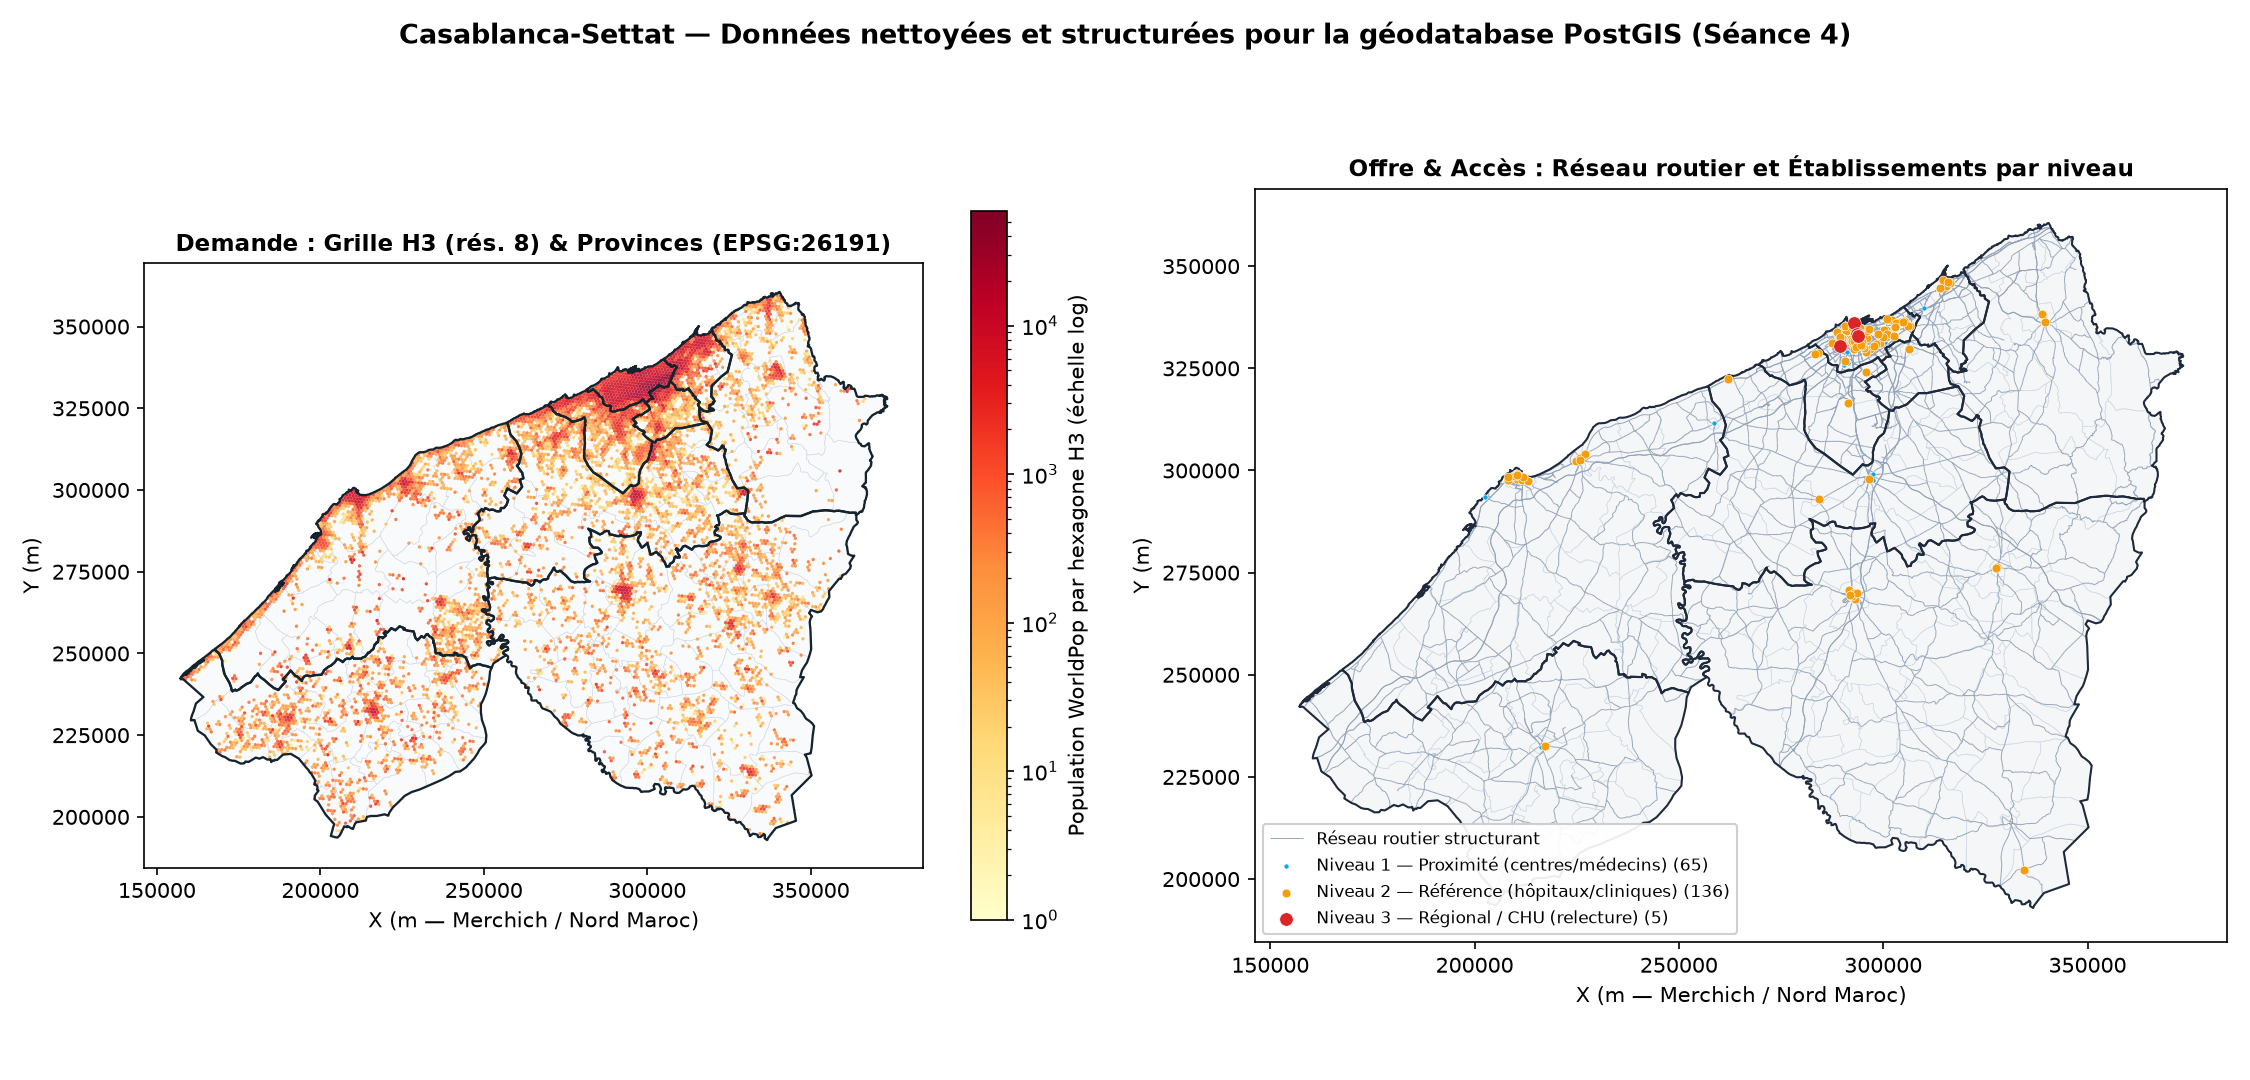
\includegraphics[width=0.95\linewidth]{carte_nettoyage.png}
\end{frame}

% =============================================================================
\partie{03}{Modèle et schéma PostGIS}{8 tables normalisées, 10 clés étrangères, contraintes CHECK et index GIST}

\begin{frame}{Architecture relationnelle et spatiale du schéma \code{sante}}
  \footnotesize
  \renewcommand{\arraystretch}{1.22}
  \begin{tabularx}{\linewidth}{@{}ll>{\raggedright\arraybackslash}Xr@{}}
    \toprule
    \textbf{Rôle} & \textbf{Table} & \textbf{Clés, géométrie (\code{EPSG:26191}) et contraintes notables} & \textbf{Lignes} \\
    \midrule
    Décision & \code{province} & PK \code{code\_province}, \code{MultiPolygon}, \code{CHECK (type\_province IN ('province','prefecture'))}, \code{ST\_IsValid} & 9 \\
    Décision & \code{commune} & PK \code{code\_hcp}, FK \code{code\_province}, \code{MultiPolygon}, \code{CHECK (pop\_2024 >= 0)}, \code{ST\_IsValid} & 153 \\
    Offre & \code{niveau\_soin} & PK \code{code\_niveau} (1, 2, 3), \code{seuil\_acces\_min} (15, 30, 60 min), \code{couvre\_niveaux\_inferieurs} & 3 \\
    Offre & \code{type\_etablissement} & PK \code{code\_type}, FK \code{niveau\_defaut}, \code{inclus\_analyse} (exclut pharmacies/dentistes/autres) & 7 \\
    Offre & \code{etablissement} & PK \code{id\_etab}, \code{osm\_id UNIQUE}, FK \code{code\_type}, \code{code\_niveau}, \code{code\_hcp}, \code{id\_noeud}, \code{Point} & 1\,583 \\
    Demande & \code{maille\_h3} & PK \code{h3\_index} (rés.\ 8), \code{population >= 0}, FK \code{code\_hcp}, \code{id\_noeud}, \code{Polygon}, \code{ST\_IsValid} & 25\,255 \\
    Accès & \code{noeud} & PK \code{id\_noeud}, \code{Point} (sommets d'intersection du graphe routier) & 228\,554 \\
    Accès & \code{troncon} & PK \code{id\_troncon}, FK \code{noeud\_depart}, \code{noeud\_arrivee} (\code{<>}), \code{longueur\_m > 0}, \code{LineString} & 318\,229 \\
    \bottomrule
  \end{tabularx}
  \vskip3mm
  \petit{Indexation complète : \textbf{6 index spatiaux GIST} sur toutes les colonnes \code{geom} + \textbf{10 index B-tree} sur toutes les clés étrangères.}
\end{frame}

% =============================================================================
\partie{04}{Requêtes métier et plans d'exécution}{Trois requêtes spatiales utiles pour la séance 5, validées par \code{EXPLAIN ANALYZE}}

\begin{frame}{Synthèse des 3 requêtes spatiales métier (\code{sql/requetes.sql})}
  \footnotesize
  \renewcommand{\arraystretch}{1.3}
  \begin{tabularx}{\linewidth}{@{}l>{\raggedright\arraybackslash}p{4.3cm}>{\raggedright\arraybackslash}Xrr@{}}
    \toprule
    \textbf{\#} & \textbf{Objectif métier (Séance 5)} & \textbf{Opérateur spatial \& Index utilisé dans \code{EXPLAIN ANALYZE}} & \textbf{Temps} \\
    \midrule
    \textbf{R1} & Diagnostic communal : population RGPH 2024 vs offre active par niveau (1, 2, 3) & \code{ST\_Within(e.geom, c.geom)} $\to$ \code{Index Scan using etablissement\_geom\_gist} & \textbf{6,5 ms} \\
    \textbf{R2} & Baseline euclidienne : plus proche établissement actif pour chaque hexagone H3 peuplé & \code{CROSS JOIN LATERAL} + KNN \code{m.geom <-> e.geom} $\to$ \code{Index Scan GIST} (7\,113 boucles) & \textbf{355,8 ms} \\
    \textbf{R3} & Connectivité routière : distance d'accrochage et densité de voirie à 2 km des hôpitaux & \code{ST\_DWithin(e.geom, tr.geom, 2000)} $\to$ \code{Index Scan using troncon\_geom\_gist} & \textbf{1\,222 ms} \\
    \bottomrule
  \end{tabularx}
  \vskip3mm
  \begin{columns}[T,onlytextwidth]
    \column{0.48\textwidth}
      \begin{tikzpicture}
        \node[fill=fond, text width=\linewidth-6mm, inner sep=2.8mm, align=left] (a)
          {{\color{sarcelle}\bfseries Résultat clé R1 (Déserts administratifs)}\\[1mm]
           \scriptsize Communes périurbaines et rurales très peuplées sans offre de niveau 1/2 : \emph{Bni Yakhlef} (117\,653 hab.), \emph{Chellalate} (98\,015 hab.), \emph{Deroua} (96\,619 hab.).};
        \fill[sarcelle] (a.north west) rectangle ($(a.south west)+(0.9mm,0)$);
      \end{tikzpicture}
    \column{0.48\textwidth}
      \begin{tikzpicture}
        \node[fill=fond, text width=\linewidth-6mm, inner sep=2.8mm, align=left] (b)
          {{\color{ambre}\bfseries Résultat clé R2 (Baseline euclidienne)}\\[1mm]
           \scriptsize Plus de \textbf{400\,000 habitants} résident dans des mailles H3 situées à plus de \textbf{10 km à vol d'oiseau} de tout établissement de soin actif (El Jadida, Berrechid, Sidi Bennour).};
        \fill[ambre] (b.north west) rectangle ($(b.south west)+(0.9mm,0)$);
      \end{tikzpicture}
  \end{columns}
\end{frame}

% =============================================================================
\partie{05}{Démonstration et suite}{Preuve d'intégrité en direct, sauvegarde restaurable et cap sur la séance 5}

\begin{frame}{Démonstration live : rejets d'intégrité et rejeu complet}
  \footnotesize
  \renewcommand{\arraystretch}{1.22}
  \begin{tabularx}{\linewidth}{@{}>{\raggedright\arraybackslash}p{5.5cm}>{\raggedright\arraybackslash}X@{}}
    \toprule
    \textbf{Test exécuté sur \code{acces\_soins}} & \textbf{Réponse immédiate de PostgreSQL / PostGIS} \\
    \midrule
    Insertion d'un établissement avec \code{code\_hcp = 'CODE\_INEXISTANT'} & \textcolor{rouge}{\code{ERROR: violates foreign key constraint "etablissement\_code\_hcp\_fkey"}} \\
    Insertion d'un point en \code{EPSG:4326} & \textcolor{rouge}{\code{ERROR: Geometry SRID (4326) does not match column SRID (26191)}} \\
    Suppression d'une commune habitée (\code{DELETE FROM commune}) & \textcolor{rouge}{\code{ERROR: update or delete on table "commune" violates FK ... (RESTRICT)}} \\
    Insertion d'un tronçon bouclant (\code{noeud\_depart = noeud\_arrivee}) & \textcolor{rouge}{\code{ERROR: violates check constraint "troncon\_noeuds\_distincts"}} \\
    \bottomrule
  \end{tabularx}
  \vskip3mm
  \commande{\scriptsize python scripts\textbackslash nettoyage.py {-}{-}dry-run \hfill\textcolor{white!55!encre}{1. diagnostic seul sans écriture}\\[0.8mm]
            python scripts\textbackslash import\_postgis.py \hfill\textcolor{white!55!encre}{2. DDL + ogr2ogr + EXPLAIN ANALYZE + pg\_dump + test pg\_restore}\\[0.8mm]
            psql -h 127.0.0.1 -U postgres -d acces\_soins -f sql\textbackslash requetes.sql \hfill\textcolor{white!55!encre}{3. exécution live des 3 requêtes}}
\end{frame}

\end{document}
